% 港式拼音 HK Pinyin for Ubuntu — manual
% Build:  xelatex hk-pinyin-manual.tex   (run twice for the table of contents)
% Needs:  texlive-xetex texlive-lang-chinese fonts-noto-cjk fonts-inter
\documentclass[11pt,a4paper]{article}

\usepackage[margin=2.2cm,top=2.4cm,bottom=2.4cm]{geometry}
\usepackage{fontspec}
\usepackage[CJKmath=true]{xeCJK}
\usepackage{xcolor}
\usepackage{graphicx}
\usepackage{booktabs}
\usepackage{tabularx}
\usepackage{array}
\usepackage{enumitem}
\usepackage{fancyvrb}
\usepackage{fvextra}
\usepackage[most]{tcolorbox}
\usepackage{tikz}
\usetikzlibrary{arrows.meta,positioning,fit,calc}
\usepackage{titlesec}
\usepackage{fancyhdr}
\usepackage{url}
\usepackage[hidelinks]{hyperref}
\urlstyle{tt}
\newfontfamily\symfont{DejaVu Sans}

% ── fonts ────────────────────────────────────────────────────────────
\setmainfont{Inter}[Scale=0.95]
\setsansfont{Inter}[Scale=0.95]
\setmonofont{DejaVu Sans Mono}[Scale=0.84]
\setCJKmainfont{Noto Sans CJK HK}[BoldFont={Noto Sans CJK HK Bold}]
\setCJKsansfont{Noto Sans CJK HK}[BoldFont={Noto Sans CJK HK Bold}]
\setCJKmonofont{Noto Sans CJK HK}
\newCJKfontfamily\serifhk{Noto Serif CJK HK}
\xeCJKsetup{CJKecglue={\hskip 0.15em plus 0.05em}}
\linespread{1.18}

% ── colours ──────────────────────────────────────────────────────────
\definecolor{accent}{HTML}{007AFF}
\definecolor{ink}{HTML}{1D1D1F}
\definecolor{muted}{HTML}{6E6E73}
\definecolor{panel}{HTML}{F5F5F7}
\definecolor{rule}{HTML}{D2D2D7}
\color{ink}

% ── headings ─────────────────────────────────────────────────────────
\titleformat{\section}{\Large\bfseries}{\color{accent}\thesection}{0.7em}{}
\titleformat{\subsection}{\large\bfseries}{\color{accent}\thesubsection}{0.6em}{}
\titlespacing*{\section}{0pt}{2.2ex}{1.2ex}
\titlespacing*{\subsection}{0pt}{1.8ex}{0.8ex}
\setlength{\parindent}{0pt}
\setlength{\parskip}{0.55em}
\setlist{itemsep=0.15em,topsep=0.3em}

\pagestyle{fancy}
\fancyhf{}
\renewcommand{\headrulewidth}{0pt}
\fancyfoot[L]{\small\color{muted}港式拼音 HK Pinyin for Ubuntu · v1.0.0}
\fancyfoot[R]{\small\color{muted}\thepage}

% ── helpers ──────────────────────────────────────────────────────────
\newcommand{\key}[1]{\tikz[baseline=(k.base)]\node[draw=rule,fill=panel,rounded corners=2.5pt,
  inner xsep=3.5pt,inner ysep=1.6pt,font=\small\ttfamily](k){#1};}
\newcommand{\code}[1]{\texttt{#1}}
\newcommand{\hk}[1]{{\large #1}}

\DefineVerbatimEnvironment{shell}{Verbatim}{breaklines,fontsize=\small}
\tcbset{codebox/.style={colback=panel,colframe=rule,boxrule=0.4pt,arc=4pt,
  left=6pt,right=6pt,top=4pt,bottom=4pt}}
\newenvironment{codeblock}{\begin{tcolorbox}[codebox]}{\end{tcolorbox}}
\newtcolorbox{note}[1][Note]{colback=accent!6,colframe=accent!60,boxrule=0.5pt,arc=4pt,
  left=7pt,right=7pt,top=4pt,bottom=4pt,fonttitle=\bfseries\small,
  title={#1},coltitle=accent!80!black,colbacktitle=accent!6,
  attach title to upper={\ \ }}

\begin{document}

% ── title ────────────────────────────────────────────────────────────
\begin{tikzpicture}[remember picture,overlay]
  \fill[panel] (current page.north west) rectangle ([yshift=-8.2cm]current page.north east);
\end{tikzpicture}
\vspace*{0.4cm}
{\fontsize{34}{40}\selectfont\bfseries 港式拼音\par}
\vspace{0.2cm}
{\LARGE HK Pinyin for Ubuntu\par}
\vspace{0.35cm}
{\large\color{muted} A macOS-style Traditional Chinese input method with Hanyu Pinyin,\\
Hong Kong glyphs, vocabulary, punctuation and date formats.\par}
\vspace{0.3cm}
{\small\color{muted} Version 1.0.0 · fcitx5 + Rime · tested on Ubuntu 24.04 LTS · 19 October 2026\par}
\vspace{1.1cm}

\begin{center}
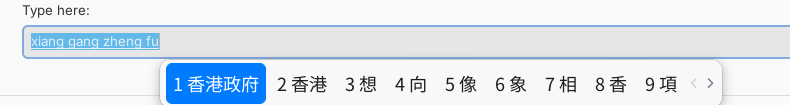
\includegraphics[width=0.8\linewidth]{img/light-sentence.png}
\end{center}

\vspace{0.4cm}
\setcounter{tocdepth}{1}
\tableofcontents

\newpage
% ════════════════════════════════════════════════════════════════════
\section{What it is}

港式拼音 is an input method for Ubuntu that behaves like the
\emph{Pinyin – Traditional} input source on macOS, but writes the way
Hong Kong writes. You type Hanyu Pinyin without tones; it gives Traditional
Chinese in a single horizontal candidate row.

\begin{center}
\renewcommand{\arraystretch}{1.25}
\begin{tabularx}{\linewidth}{@{}>{\bfseries}p{3.4cm}X@{}}
\toprule
Input & Hanyu Pinyin, full syllables or initials (\code{xg} → 香港), whole-sentence conversion, learns the words you choose. \\
Characters & Hong Kong forms: 為 衞 線 枱 啟 群 眾, keeping the Big5 code points used on HK websites (戶 說 稅). \\
Vocabulary & Hong Kong terms first: 軟件 網絡 的士 雪櫃 電郵 甚麼. 376 built-in HK words, place names and written-Cantonese words (嘅 咗 佢哋 唔該). \\
Punctuation & 「」 『』 、 ， 。 …… —— 《》, all on the keys a macOS user expects. \\
Dates & \code{rq} 2026年10月19日 · 19/10/2026; \code{sj} 下午3:05; \code{xq} 星期一. \\
Look \& keys & macOS light and dark candidate windows; \key{Ctrl+Space} switches input source; \key{Shift} toggles English. \\
\bottomrule
\end{tabularx}
\end{center}

\subsection{How it is built}

There is no new C code in the typing path. 港式拼音 is a Rime \emph{schema}
running inside fcitx5, the standard input-method framework on Ubuntu, so it
gets fcitx5's support for GTK, Qt, X11 and Wayland applications for free.

\begin{center}
\begin{tikzpicture}[
  box/.style={draw=rule,fill=panel,rounded corners=4pt,minimum height=0.9cm,
              text width=3.1cm,align=center,font=\small},
  hk/.style={box,draw=accent,fill=accent!7},
  arr/.style={-{Stealth[length=2.2mm]},thick,color=muted},
  node distance=0.55cm and 0.6cm]
  \node[box] (kb) {Keyboard\\\code{xianggang}};
  \node[box,right=of kb] (fx) {fcitx5\\\scriptsize key routing, window};
  \node[box,right=of fx] (sp) {Rime speller\\\scriptsize pinyin syllables};
  \node[hk,below=0.9cm of sp] (tr) {Translators\\\scriptsize hk\_pinyin dictionary\\ + hk\_datetime.lua};
  \node[hk,left=of tr] (tf) {hk\_terms\_filter\\\scriptsize 冰箱 → 雪櫃 | 冰箱};
  \node[hk,left=of tf] (gf) {hk\_glyph\\\scriptsize 爲 → 為, 衛 → 衞};
  \node[hk,below=0.9cm of gf] (ui) {macOS theme\\\scriptsize 1 香港 2 想 3 向 …};
  \node[box,right=of ui] (app) {Application\\\scriptsize receives 香港};
  \draw[arr] (kb) -- (fx); \draw[arr] (fx) -- (sp); \draw[arr] (sp) -- (tr);
  \draw[arr] (tr) -- (tf); \draw[arr] (tf) -- (gf); \draw[arr] (gf) -- (ui);
  \draw[arr] (ui) -- (app);
  \node[font=\scriptsize\color{accent},anchor=west] at ([xshift=2mm]tr.east) {this project};
\end{tikzpicture}
\end{center}

The dictionary \code{hk\_pinyin} is Rime's 朙月拼音 (\code{luna\_pinyin}) word
list, plus the Hong Kong word list, plus your own words. Two filters then
rewrite each candidate: the first puts the Hong Kong term ahead of the
mainland or Taiwan term, the second changes inherited character forms to
the Hong Kong ones.

% ════════════════════════════════════════════════════════════════════
\section{Install}

\subsection{Requirements}
\begin{itemize}
  \item Ubuntu 24.04 LTS (tested) or newer, or Debian 12+. Ubuntu 22.04 works
        with a fallback: without \code{librime-plugin-lua} you lose the \code{rq}/\code{sj}
        date shortcuts, and Hong Kong terms replace the original instead of being listed first.
  \item GNOME, KDE Plasma, Xfce or any other desktop. Both X11 and Wayland.
  \item About 60 MB of packages if fcitx5 is not already installed.
\end{itemize}

\subsection{Steps}
Download the project and run the installer \emph{as yourself} (it calls \code{sudo} only for \code{apt}):

\begin{codeblock}
\begin{shell}
git clone https://github.com/YOUR-USERNAME/hk-pinyin-ime.git
cd hk-pinyin-ime
./install.sh
\end{shell}
\end{codeblock}

The installer:
\begin{enumerate}
  \item installs fcitx5, fcitx5-rime, the luna\_pinyin data, librime-lua and the Noto CJK HK fonts;
  \item copies the schema, dictionaries, Lua scripts and OpenCC tables to \path{~/.local/share/fcitx5/rime/} and compiles them;
  \item installs the \code{macos-light} and \code{macos-dark} themes;
  \item sets up fcitx5: English + 港式拼音, \key{Ctrl+Space} to switch, horizontal candidates, Noto Sans CJK HK, input state shared across windows;
  \item makes fcitx5 the system input method (\code{im-config}, \code{environment.d}, autostart).
\end{enumerate}
Any fcitx5 settings it replaces are copied to \path{~/.config/fcitx5/hk-pinyin-backup-<date>/} first.

\textbf{Then log out and log back in once.}

\begin{note}[GNOME on Wayland]
Install the GNOME Shell extension \emph{Input Method Panel} (kimpanel) from
\code{extensions.gnome.org}. Without it the candidate window may appear at a corner
of the screen instead of under the cursor in some applications.
\end{note}

\subsection{Options}
\begin{center}
\begin{tabularx}{\linewidth}{@{}>{\ttfamily}lX@{}}
\toprule
--no-apt & Do not install packages (you already have fcitx5 and fcitx5-rime). \\
--layout gb & Keyboard layout for the English input source. Default: detected, otherwise \code{us}. \\
--no-config & Only install the schema and themes; keep your fcitx5 settings. Add 港式拼音 yourself in \emph{Fcitx 5 Configuration}. \\
\bottomrule
\end{tabularx}
\end{center}

% ════════════════════════════════════════════════════════════════════
\section{Using it}

\subsection{Keys}
\begin{center}
\renewcommand{\arraystretch}{1.35}
\begin{tabularx}{\linewidth}{@{}l X X@{}}
\toprule
\textbf{Key} & \textbf{港式拼音 on Ubuntu} & \textbf{macOS equivalent} \\
\midrule
\key{Ctrl+Space} & Switch English {\symfont ⇄} 港式拼音 & \key{Ctrl+Space} \\
\key{Shift} & Toggle English inside 港式拼音; letters already typed are entered as English & \key{Caps Lock} / \key{Shift} \\
\key{Space} \key{1}–\key{9} & Choose a candidate & same \\
\key{-} \key{=} \key{Tab} & Previous / next page & same \\
\key{←} \key{→} & Move through candidates & same \\
\key{Enter} & Enter the letters as typed & same \\
\key{Esc} & Cancel & same \\
\key{Ctrl+`} or \key{F4} & Options menu (below) & — \\
\key{Shift+Space} & Half-width {\symfont ⇄} full-width & — \\
\key{Ctrl+.} & Chinese {\symfont ⇄} English punctuation & — \\
\bottomrule
\end{tabularx}
\end{center}

Type a capital letter first (\code{Hello}) to write English directly without switching.
Type \code{/} and a code for symbols: \code{/fh} © ® ™, \code{/jt} arrows, \code{/sx} maths.

\subsection{Options menu}
\key{Ctrl+`} opens the options. Your choices are remembered.
\begin{center}
\begin{tabular}{@{}lll@{}}
\toprule
\textbf{Option} & \textbf{On (default)} & \textbf{Off} \\
\midrule
香港詞彙 & 雪櫃 first, 冰箱 second & 冰箱 only \\
香港字形 & 為 衞 線 & 爲 衛 綫 (Rime's inherited forms) \\
全形 / 半形 & — & half-width (default) \\
中文標點 & 「，。」 & ASCII punctuation \\
\bottomrule
\end{tabular}
\end{center}

\subsection{What it looks like}
\newcommand{\shot}[3]{\par\noindent\begin{minipage}{\linewidth}\centering
  \includegraphics[width=#1]{#2}\\[0.1em]{\small\color{muted}#3}\end{minipage}\par\vspace{0.8em}}
\shot{0.72\linewidth}{img/light-terms.png}{Hong Kong term first, the mainland/Taiwan word right after: \code{bingxiang} → 1\,雪櫃 2\,冰箱}
\shot{\linewidth}{img/light-date.png}{\code{rq} gives today's date in Hong Kong formats}
\shot{0.72\linewidth}{img/dark-terms.png}{The dark theme follows the desktop's dark mode: \code{weishenme} → 為甚麼}

% ════════════════════════════════════════════════════════════════════
\section{Hong Kong conventions}

\subsection{Characters}
Rime's dictionary stores inherited (舊字形) forms. The \code{hk\_glyph} filter changes them to
the forms in everyday Hong Kong use — the ones on government websites, in newspapers and
produced by Big5/HKSCS input methods such as 倉頡 and 速成.

\begin{center}
\renewcommand{\arraystretch}{1.2}
\begin{tabular}{@{}*{8}{c}@{}}
\toprule
爲→\hk{為} & 衛→\hk{衞} & 綫→\hk{線} & 檯→\hk{枱} & 啓→\hk{啟} & 羣→\hk{群} & 衆→\hk{眾} & 裡→\hk{裏} \\
牀→\hk{床} & 峯→\hk{峰} & 敘→\hk{敍} & 鉤→\hk{鈎} & 蔥→\hk{葱} & 菸→\hk{煙} & 卧→\hk{臥} & 麪→\hk{麵} \\
\bottomrule
\end{tabular}
\end{center}

Characters such as 戶 說 稅 脫 溫 are deliberately \emph{not} changed to 户 説 税 脱 温.
Those are the shapes in the 常用字字形表 reference, but Hong Kong text uses the
Big5 code points and lets the HK font draw the local shape. If you want the strict reference
forms, see \S\ref{sec:strict}.

\subsection{Vocabulary}
Hong Kong words are in the dictionary with high weights, and a filter rewrites mainland or
Taiwan terms inside any candidate, sentence or phrase, while keeping the original as the next choice.

\begin{center}
\renewcommand{\arraystretch}{1.18}
\begin{tabular}{@{}lll@{\hspace{2.2em}}lll@{}}
\toprule
\textbf{You type} & \textbf{First} & \textbf{Instead of} & \textbf{You type} & \textbf{First} & \textbf{Instead of} \\
\midrule
ruanjian & 軟件 & 軟體 & dishi & 的士 & 計程車 \\
wangluo & 網絡 & 網路 & bashi & 巴士 & 公車 \\
dayinji & 打印機 & 印表機 & bingxiang & 雪櫃 & 冰箱 \\
shujuku & 數據庫 & 資料庫 & lianjie & 連結 & 鏈接 \\
dianyou & 電郵 & 電子郵件 & zhuguli & 朱古力 & 巧克力 \\
duanxun & 短訊 & 簡訊 / 短信 & xuegao & 雪糕 & 冰淇淋 \\
shangzai & 上載 & 上傳 & sanwenzhi & 三文治 & 三明治 \\
shuma & 數碼 & 數位 & danche & 單車 & 腳踏車 \\
rengongzhineng & 人工智能 & 人工智慧 & jiemian & 介面 & 界面 \\
shenme & 甚麼 & 什麼 & anjie & 按揭 & 房貸 \\
\bottomrule
\end{tabular}
\end{center}

The built-in list also covers government bodies (立法會, 廉政公署, 食環署, 強積金),
housing (公屋, 居屋, 劏房), transport (港鐵, 八達通, 小巴), about 70 districts
(旺角, 尖沙咀, 鰂魚涌, 赤鱲角) and common written-Cantonese characters and words
(嘅 咗 喺 唔 冇 佢 哋 嘢 · 唔該 我哋 而家 點解 搞掂). For these, a sensible Mandarin
reading is used: 佢 \code{qu}, 嘅 \code{ge}, 冇 \code{mao}, 喺 \code{xi}, 嘢 \code{ye}, 哋 \code{di}.

Where a Hong Kong word shares its pinyin with a very common word, the common word stays first
(\code{zhishi} → 只是, then 芝士). After you choose 芝士 a few times, it moves up for you.

\subsection{Punctuation}
\begin{center}
\renewcommand{\arraystretch}{1.25}
\begin{tabular}{@{}cc@{\hspace{1.5em}}cc@{\hspace{1.5em}}cc@{\hspace{1.5em}}cc@{}}
\toprule
\textbf{Key} & \textbf{Gives} & \textbf{Key} & \textbf{Gives} & \textbf{Key} & \textbf{Gives} & \textbf{Key} & \textbf{Gives}\\
\midrule
\key{,} & ， & \key{[} & 「 & \key{"} & 「 then 」 & \key{\textbackslash} & 、 \\
\key{.} & 。 & \key{]} & 」 & \key{'} & 『 then 』 & \key{\textasciicircum} & …… \\
\key{?} & ？ & \key{\{} & 『 & \key{<} & 《 〈 « & \key{\_} & —— \\
\key{!} & ！ & \key{\}} & 』 & \key{>} & 》 〉 » & \key{\$} & \$ HK\$ ¥ € £ \\
\key{;} & ； & \key{(} & （ & \key{:} & ： & \key{*} & * × ※ \\
\bottomrule
\end{tabular}
\end{center}
Keys with several choices (\key{<}, \key{\$}, \key{*}) show a small menu; press the key again or a number.

\subsection{Dates and times}
\begin{center}
\renewcommand{\arraystretch}{1.25}
\begin{tabularx}{\linewidth}{@{}>{\ttfamily}lX@{}}
\toprule
rq & 2026年10月19日 · 19/10/2026 · 二〇二六年十月十九日 · 2026-10-19 \\
sj & 下午3:05 · 15:05 · 下午三時零五分 (三時正 on the hour) \\
xq & 星期一 · 週一 · （一） \\
dt & 2026年10月19日（星期一）下午3:05 · 19/10/2026 15:05 \\
\bottomrule
\end{tabularx}
\end{center}
Numeric dates are day/month/year, as in Hong Kong. Periods are 凌晨, 上午, 下午, 晚上.

% ════════════════════════════════════════════════════════════════════
\section{Customising}
All customisation lives in \path{~/.local/share/fcitx5/rime/}. After a change,
choose \emph{Deploy} (重新部署) in the fcitx5 tray menu, or run \code{fcitx5 -r}.
Reinstalling never overwrites your own files:
\begin{itemize}
  \item \code{hk\_pinyin.user\_terms.dict.yaml} — your words;
  \item \code{hk\_pinyin.custom.yaml} — your settings (only on systems without librime-lua does the installer write it, after making a backup).
\end{itemize}

\subsection{Add your own words}
Edit \code{hk\_pinyin.user\_terms.dict.yaml}. Below the \code{...} line, one word per line,
separated by \emph{Tab} characters: word, pinyin, weight.
\begin{codeblock}
\begin{shell}
長洲太平清醮	chang zhou tai ping qing jiao	50000
將軍澳中心	jiang jun ao zhong xin	50000
\end{shell}
\end{codeblock}
Use \code{v} for ü (\code{lv} 律, \code{nv} 女). A weight of 50000 puts a word ahead of most homophones.

\subsection{Common changes}
Create \code{hk\_pinyin.custom.yaml} with any of these under \code{patch:}.
\begin{codeblock}
\begin{shell}
patch:
  # fewer candidates per page
  menu/page_size: 6

  # fuzzy pinyin: z=zh c=ch s=sh, an=ang en=eng in=ing
  speller/algebra/+:
    - derive/^([zcs])h/$1/
    - derive/^([zcs])([^h])/$1h$2/
    - derive/([aei])n$/$1ng/
    - derive/([aei])ng$/$1n/

  # start each window in English instead of Chinese
  switches/@0/reset: 1
\end{shell}
\end{codeblock}

\subsection{Strict 常用字字形表 character forms}\label{sec:strict}
To get 户 説 税 温 and the other reference shapes, copy OpenCC's \code{t2hk} tables and point
the glyph filter at them:
\begin{codeblock}
\begin{shell}
cp /usr/share/opencc/t2hk.json /usr/share/opencc/HKVariants.ocd2 \
   ~/.local/share/fcitx5/rime/opencc/
\end{shell}
\end{codeblock}
\begin{codeblock}
\begin{shell}
patch:
  hk_glyph/opencc_config: t2hk.json
\end{shell}
\end{codeblock}

\subsection{Window style}
\emph{Fcitx 5 Configuration} → \emph{Addons} → \emph{Classic User Interface}: choose
\code{macos-light} / \code{macos-dark}, the font, or a vertical list. To change colours, edit
\code{THEMES} in \code{tools/make\_themes.py}, run it, and run \code{./install.sh --no-apt} again.

% ════════════════════════════════════════════════════════════════════
\section{Project files}
\begin{center}
\renewcommand{\arraystretch}{1.18}
\begin{tabularx}{\linewidth}{@{}>{\ttfamily\small}lX@{}}
\toprule
install.sh, uninstall.sh & Installer and remover. \\
rime/hk\_pinyin.schema.yaml & The schema: switches, engine pipeline, punctuation, keys. \\
rime/hk\_pinyin.dict.yaml & Main dictionary: imports luna\_pinyin + HK terms + user terms. \\
rime/hk\_pinyin.hk\_terms.dict.yaml & 376 Hong Kong words (generated). \\
rime/hk\_pinyin.user\_terms.dict.yaml & Your words (installed once, never overwritten). \\
rime/default.custom.yaml & Global Rime settings: page size, Shift behaviour, menu keys. \\
rime/lua/hk\_datetime.lua & \code{rq} \code{sj} \code{xq} \code{dt}. \\
rime/lua/hk\_terms\_filter.lua & Puts Hong Kong terms first, keeps the original next. \\
rime/opencc/hk\_terms.txt & Mainland/Taiwan → Hong Kong term pairs. \\
rime/opencc/hk\_glyph.txt & Inherited → Hong Kong character forms. \\
themes/macos-light, macos-dark & fcitx5 themes (generated). \\
tools/hk\_terms.src, build\_dict.py & Source of the HK word list and its generator (checks syllable counts). \\
tools/make\_themes.py & Draws the theme images and writes \code{theme.conf}. \\
tests/rime\_probe.c, run\_tests.sh & Types pinyin into librime and checks 26 expected results. \\
docs/ & This manual (\code{.tex} and \code{.pdf}). \\
\bottomrule
\end{tabularx}
\end{center}

\subsection{Development loop}
\begin{codeblock}
\begin{shell}
sudo apt install gcc librime-dev librime-plugin-lua rime-data-luna-pinyin python3-pil
vim tools/hk_terms.src            # add words:  詞語 | pin yin | weight
python3 tools/build_dict.py       # regenerate the dictionary
tests/run_tests.sh                # 26 checks, no desktop needed
./install.sh --no-apt             # try it for real
\end{shell}
\end{codeblock}

% ════════════════════════════════════════════════════════════════════
\section{Troubleshooting}
\renewcommand{\arraystretch}{1.3}
\begin{tabularx}{\linewidth}{@{}>{\raggedright\arraybackslash}p{4.6cm}>{\raggedright\arraybackslash}X@{}}
\toprule
\textbf{Problem} & \textbf{Fix} \\
\midrule
Ctrl+Space does nothing & Log out and in after installing. Check \code{im-config -m} shows \code{fcitx5}, and that \code{fcitx5} is running (\code{pgrep fcitx5}). \\
Works in some apps, not others & Install \code{fcitx5-frontend-gtk4} / \code{fcitx5-frontend-qt6}. For Flatpak apps: \code{flatpak override --user --env=GTK\_IM\_MODULE=fcitx}. \\
Candidate window in a screen corner (GNOME Wayland) & Install the kimpanel GNOME extension. \\
Chromium / Electron apps on Wayland & Start with \code{--enable-wayland-ime}, or run them under XWayland. \\
No \code{rq} dates; terms replaced not listed & \code{librime-plugin-lua} is missing; install it and run \code{./install.sh --no-apt}. \\
Changes to word lists have no effect & Tray menu → \emph{Deploy}, or \code{fcitx5 -r}. Check \code{/tmp/hk-pinyin-deploy.log}. \\
A wrong word keeps coming first & Select the right one a few times; Rime learns. To forget learned words: \code{./uninstall.sh --purge} and reinstall. \\
\bottomrule
\end{tabularx}

% ════════════════════════════════════════════════════════════════════
\section{Removing}
\begin{codeblock}
\begin{shell}
./uninstall.sh          # remove schema and themes, keep learned words
./uninstall.sh --purge  # also delete learned words and your word list
im-config -n ibus       # optional: go back to IBus
\end{shell}
\end{codeblock}

% ════════════════════════════════════════════════════════════════════
\section{Known limits}
\begin{itemize}
  \item \key{Caps Lock} types capital letters; it does not switch input sources as on macOS
        (Linux has no clean way to stop Caps Lock also toggling capitals). Use \key{Shift}.
  \item There is no cloud or AI prediction. Conversion uses Rime's statistical model and your history.
  \item How the not-yet-converted pinyin looks inside the text field (underlined or highlighted)
        depends on the application.
  \item Written-Cantonese characters are typed with approximate Mandarin readings, not Jyutping.
        For full Cantonese input, add Rime's \code{jyut6ping3} schema alongside.
  \item Tested with Ubuntu 24.04, fcitx5 5.1.7, librime 1.10, librime-lua 2023-09.
\end{itemize}

\vfill
{\small\color{muted} Built on fcitx5 (LGPL-2.1), librime and luna\_pinyin (BSD-3-Clause/LGPL-3.0),
librime-lua (BSD-3-Clause), OpenCC (Apache-2.0) and Noto CJK fonts (OFL-1.1).\par}

\end{document}
